\documentclass{beamer}
\usepackage[export]{adjustbox}
\DeclareMathOperator*{\argmax}{arg\,max}

\usetheme{metropolis}           % Use metropolis theme
\title{The Bayesian Occam's razor for the hierarchical clustering of MSM's}
\date{\today}
\author{Ben Harland}
% \institute{Centre for Modern Beamer Themes}

\begin{document}
\maketitle

\begin{frame}{Occam's razor}
\begin{columns}[T,onlytextwidth]
\column{0.7\textwidth}
\begin{block}{}
``Entities should not be multiplied without necessity.''
\end{block}
\begin{block}
{\small William of Ockham (c. 1287–1347)}
\end{block}
\begin{block}{}
``Everything should be made as simple as possible, but no simpler.''
\end{block}
\begin{block}
{\small Einstein (New York Times, 1950)}
\end{block}
% \begin{block}{}
% ``It can scarcely be denied that the supreme goal of all theory is to
% make the irreducible basic elements as simple and as few as possible without
% having to surrender the adequate representation of a single datum of experience.''
% \end{block}
% \begin{block}
% {\small Einstein (The Ultimate Quotable Einstein)}
% \end{block}
\column{0.3\textwidth}
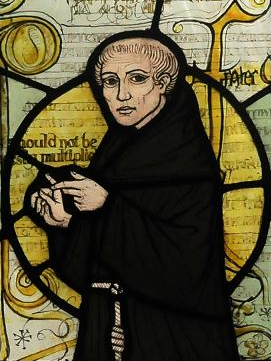
\includegraphics[width=\textwidth]{figures/William_of_Ockham.png}
\end{columns}
\begin{block}{}
``It can scarcely be denied that the supreme goal of all theory is to
make the irreducible basic elements as simple and as few as possible without
having to surrender the adequate representation of a single datum of experience.''
\end{block}
\begin{block}
{\small The Ultimate Quotable Einstein}
\end{block}
\end{frame}

\begin{frame}{Helpful books (youtube)}{}
\begin{tabular}{ll}
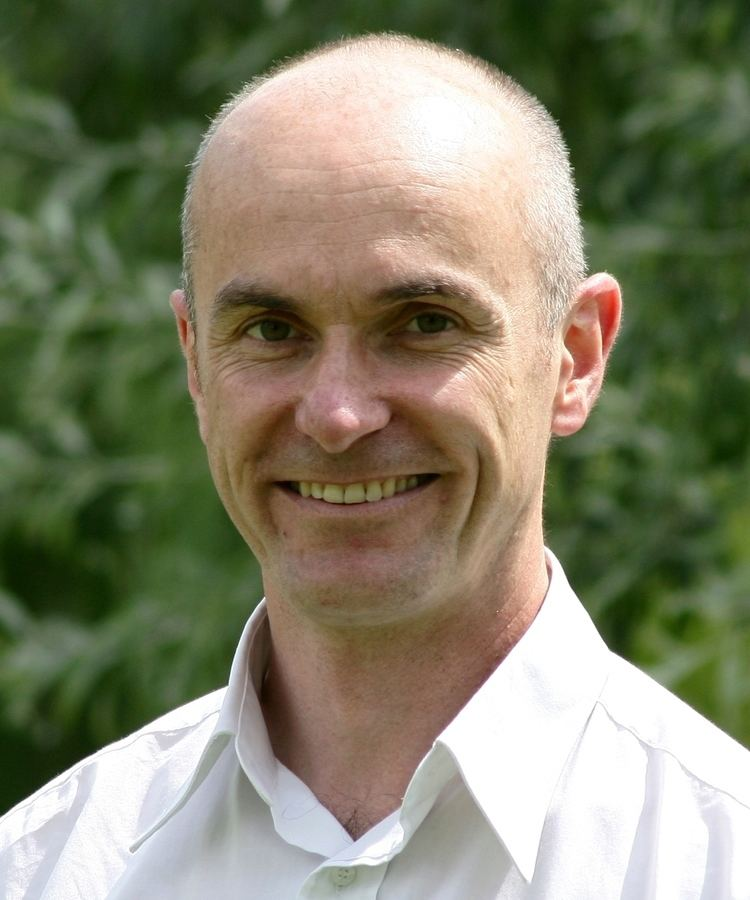
\includegraphics[width=0.4\textwidth]{figures/david-j-c-mackay.jpeg} &
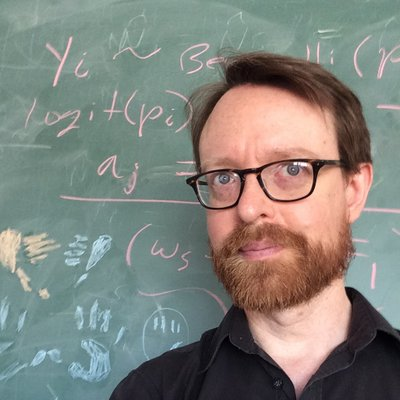
\includegraphics[width=0.4\textwidth]{figures/mcelreath.jpg} \\
David MacKay & Richard McElreath \\
{\tiny Information Theory, Inference, and Learning Algorithms} &
{\tiny Statistical Rethinking}
\end{tabular}{}
\end{frame}

\begin{frame}{Hierarchical protein dynamics}{}
\begin{figure}
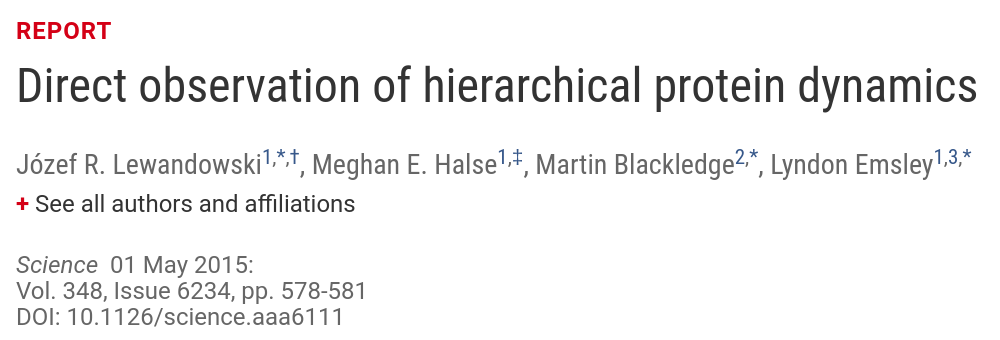
\includegraphics[width=0.6\textwidth]{figures/lewandowski-title.png}{}
\end{figure}
\begin{figure}
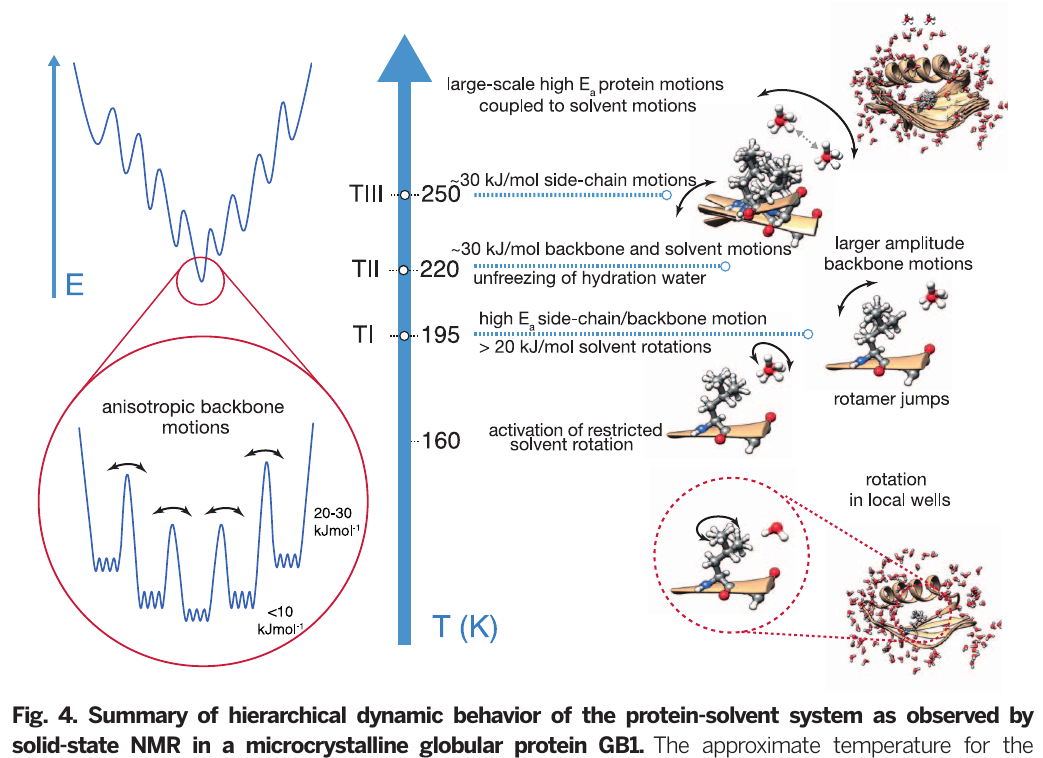
\includegraphics[width=0.6\textwidth]{figures/lewandowski-figure.png}
\end{figure}
\end{frame}

\begin{frame}{Markov models}
\begin{tabular}{ll}
\textrm{Microstates (or macrostates)} & \textrm{Macrostate/microstate model} \\
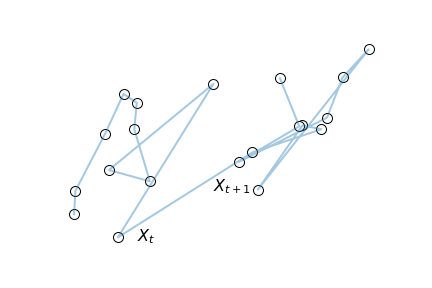
\includegraphics[width=0.5\textwidth]{figures/msm-microstates.png} &
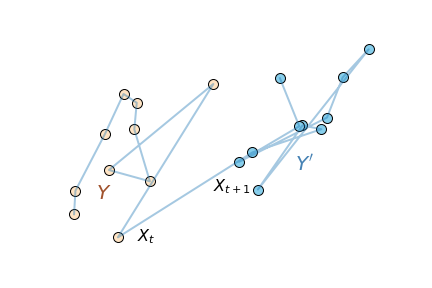
\includegraphics[width=0.5\textwidth]{figures/msm-macrostates.png} \\
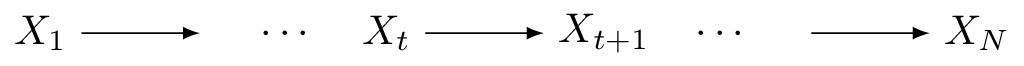
\includegraphics[width=0.5\textwidth]{figures/tikzmicrostates.png} &
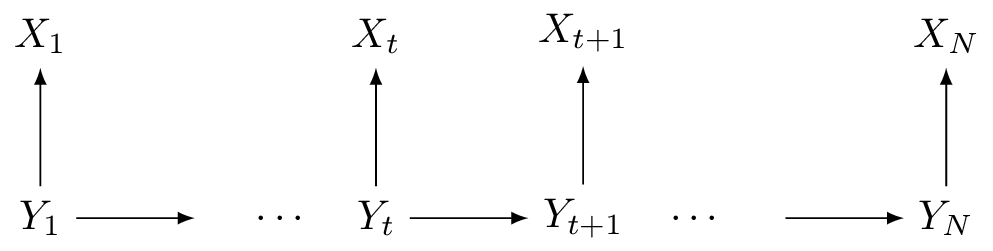
\includegraphics[width=0.5\textwidth]{figures/tikzmacrostates.png} \\
\scalebox{0.8}{$P(X_{t+1}=x_j|X_t=x_i) = T_{ij}$} &
\scalebox{0.8}{$P(X_{t+1}=x_\nu, Y_{t+1}=y_j|Y_t=y_i) = T_{ij}\theta_{j,\nu}$}
\end{tabular}
\end{frame}

\begin{frame}{Likelihood}
Model
\[
x \in \{x_i\}_{i=1}^n
\]
Data
\[ x_N \equiv x_1, x_2, \ldots, x_N \]
Likelihood
\[ P(x_N|T, M) \approx \prod_{i=1}^{N-1} T_{x_i,x_{i+1}} \]
Go to transition counts
\[ P(C|T, M) \approx \prod_{i=1}^n\prod_{j=1}^n T_{ij}^{C_{ij}} \]
\end{frame}

\begin{frame}{Maximum likelihood}
Maximum likelihood estimate
\[ \hat{T} = \argmax\Big\{P(C|T,M) \Big| \sum_j T_{ij}=1\forall i \Big\}\]
\[ \hat{T}_{ij} = \frac{C_{ij}}{C_i} ~~~~~ C_i = \sum_j C_{ij}\]
Maximum likelihood
\[ \log P(C|\hat{T},M) = \sum_{i=1}^n\sum_{j=1}^n C_{ij}\log\frac{C_{ij}}{C_i} \]
\end{frame}

\begin{frame}{Bayesian inference}
Type I inference: posterior distribution
\[ P(T|C,M) = \frac{P(C|T,M)P(T|M)}{P(C|M)} \]
Type II inference: model comparison
\[ P(M|C) = \frac{P(C|M) P(M)}{P(C)} \]
Evidence
\[ P(C|M) = \int_T P(C,T|M)
= \int_T \underbrace{P(C|T,M)}_{\prod_{i,j}T_{ij}^{C_{ij}}}
\underbrace{P(T|M)}_{\prod_i\frac{\Gamma(A_i)}{\prod_j\Gamma(\alpha_{ij})}\prod_j T_{ij}^{\alpha_{ij}-1}} \]
\end{frame}

\begin{frame}{Evidence}
Analytical result (symmetric prior, $\alpha_{ij}=1/n$)
\[ P(C|M) \approx \sum_{j=1}^n C_{ij}\log\frac{C_{ij}}{C_i} -n^2\log n \]
Laplace estimate
\[ P(C|M) = \int_T P(C,T|M) \sim
\underbrace{P(C, \hat{T}|M)}_{\propto P(T|C,M)} \times \sigma_{C,T} \]
\begin{columns}[T,onlytextwidth]
\column{0.4\textwidth}
{\small ``For many problems, the posterior has a strong peak at the most probable
parameters.'' -- Mackay, \emph{Information Theory}, p. 348}
\column{0.6\textwidth}
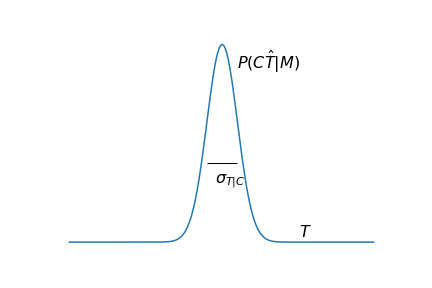
\includegraphics[width=\textwidth]{figures/PCT-dist.png}
\end{columns}
\end{frame}

\begin{frame}{Occam's razor}
\begin{align*}
P(C|M) &\sim P(C, \hat{T}|M) \times \sigma_{T|C} \\
&= \underbrace{P(C|\hat{T},M)}_{\sim\textrm{max likelihood}}
\underbrace{P(\hat{T}|M)}_{\sim \sigma_T^{-1}}
\times\sigma_{T|C}
\end{align*}
Occam factor:
\[ \log\frac{\sigma_{T|C}}{\sigma_T} \sim -n^2\log n \]
\begin{itemize}
    \item $\sigma_{T|C}/\sigma_T < 1$ is the penalty to the evidence for
    choosing a prior that is broad relative to the volume of parameter space
    that captures the peak of the joint distribution (at data = $C$).
    \item "The factor by which $M$'s hypothesis space collapses when the
    data arrive"
\end{itemize}
\end{frame}

\begin{frame}
\end{frame}

\begin{frame}
\end{frame}

\begin{frame}
\end{frame}

\begin{frame}
\end{frame}
\end{document}
